\problemname{Portals}

The new company Sweden Portal Transit wants to revolutionize how Swedish
commuters get around the country. The company has put forward
a groundbreaking proposal for how a portal system should be built in Sweden, to
replace trains, flights, and bus services with fuel-efficient portals. The government
has now been tasked with reviewing the proposal in detail, and is appealing to
Swedish elite programmers for help. This is where you come in.

You have been given access to a blueprint of the portal system to analyze it.
The portal system consists of $N$ portals placed at various locations in the country. Each portal $a$
has a certain destination portal $b$. This means that every time you enter $a$ you come
out of $b$. Note that you do not necessarily return to $a$ when you enter $b$.
Sweden Portal Transit's new idea is that by letting travelers enter
a portal and then repeatedly enter the portal they emerge from, they will quickly
be able to get around the country.

The government now wants to know, for a number of given start and end portals $a$ and $b$,
how many times one needs to enter the portal one emerges from to get from $a$ to
$b$ -- or if it is even possible. For each such query you should answer with the number of
times one needs to enter portals to get from $a$ to $b$. If it is impossible
you should answer $-1$.

Help the government!

\section*{Input}

The first line of input contains the integer $N$, the number of portals that will be placed in the country.
Then follow $N$ lines with numbers $1 \le d_i \le N$ describing that the portal on line $i$ leads to portal $d_i$.
The portals are one-indexed (the lowest has number 1, the highest has number $N$), and come in order from $1$ to $N$ in the input.

Then follows a line with an integer $Q$, the number of queries you must answer. After that
follow $Q$ lines with two integers $1 \le s, e \le N$. These numbers describe the number of a start portal $s$ and an
end portal $e$, and your task is to answer how many times one needs to go through portals
to reach $e$ when starting at $s$. For each query, $s \neq e$.

\section*{Output}
You should output $Q$ lines, one number per query: the number of times one needs to go
through portals to get from the given start portal to the
end portal. If it is impossible, output $-1$. Output the answer
for each query on a separate line.

\section*{Explanation of Samples}

\begin{figure}[ht!]
\centering
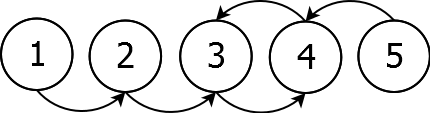
\includegraphics[width=0.4\textwidth]{portaler.png}
\caption{An illustration of Sample Input 1.}
\label{overflow}
\end{figure}

The network in the sample looks like the figure. We get three queries. The first
asks how many times we need to enter portals when starting at $1$ and wanting to end up
at $2$. Since we immediately arrive at $2$ when we enter $1$, the answer is $1$. To
get from $1$ to $4$ requires three hops. For the last query the answer is $-1$,
since we can never get from $2$ to $5$, no matter how long we keep going through portals.

\section*{Scoring}
Your solution will be tested on a set of test groups. To earn points for a group,
you must pass all test cases in that group.

\begin{tabular}{| l | l | l | l |}
\hline
Group & Points & Constraints & Other\\ \hline
1     & 10         & $ 1 \le N \le 1\,000,\ 1 \le Q \le 1\,000$ & There will always be a path between the start and end portals.\\ \hline
2     & 20         & $ 1 \le N \le 1\,000,\ 1 \le Q \le 1\,000$ &  \\ \hline
3     & 10         & $ 1 \le N \le 7\,000,\ 1 \le Q \le 120\,000$ & There will always be a path between the start and end portals.\\ \hline
4     & 10         & $ 1 \le N \le 7\,000,\ 1 \le Q \le 120\,000$ &  \\ \hline
5     & 10         & $ 1 \le N \le 50\,000,\ 1 \le Q \le 70\,000$ & There will always be a path between the start and end portals. The test cases are also a bit easier than group 6.\\ \hline
6     & 30         & $ 1 \le N \le 50\,000,\ 1 \le Q \le 70\,000$ & There will always be a path between the start and end portals. \\ \hline
7     & 10         & $ 1 \le N \le 50\,000,\ 1 \le Q \le 70\,000$ &  \\ \hline
\end{tabular}
